\documentclass[a4paper,14pt]{extarticle}

\usepackage[utf8x]{inputenc}
\usepackage[T1]{fontenc}
\usepackage[russian]{babel}
\usepackage{hyperref}
\usepackage{indentfirst}
\usepackage{here}
\usepackage{array}
\usepackage{graphicx}
\usepackage{caption}
\usepackage{subcaption}
\usepackage{chngcntr}
\usepackage{amsmath}
\usepackage{amssymb}
\usepackage[left=2cm,right=2cm,top=2cm,bottom=2cm,bindingoffset=0cm]{geometry}
\usepackage{multicol}
\usepackage{multirow}
\usepackage{titlesec}
\usepackage{listings}
\usepackage{color}
\usepackage{enumitem}
\usepackage{cmap}
\usepackage{url}

\definecolor{green}{rgb}{0,0.6,0}
\definecolor{gray}{rgb}{0.5,0.5,0.5}
\definecolor{purple}{rgb}{0.58,0,0.82}

\lstdefinelanguage{none}{}

\lstset{
	language={none},
	inputpath={../logs/},
	backgroundcolor=\color{white},
	commentstyle=\color{green},
	keywordstyle=\color{blue},
	numberstyle=\color{gray}\scriptsize\ttfamily,
	stringstyle=\color{purple},
	basicstyle=\footnotesize\ttfamily,
	breakatwhitespace=false,
	breaklines=true,
	captionpos=b,
	keepspaces=true,
	numbers=left,
	numbersep=5pt,
	showspaces=false,
	showstringspaces=false,
	showtabs=false,
	tabsize=4,
	frame=single,
	morekeywords={},
	deletekeywords={},
	extendedchars=false,
	columns=fullflexible,
	literate=%
		{~}{{\raise.25ex\hbox{$\mathtt{\sim}$}}}{1}%
		{-}{-}{1}
}

\titleformat*{\section}{\large\bfseries} 
\titleformat*{\subsection}{\normalsize\bfseries} 
\titleformat*{\subsubsection}{\normalsize\bfseries} 
\titleformat*{\paragraph}{\normalsize\bfseries} 
\titleformat*{\subparagraph}{\normalsize\bfseries} 

\counterwithin{figure}{section}
\counterwithin{equation}{section}
\counterwithin{table}{section}
\newcommand{\sign}[1][5cm]{\makebox[#1]{\hrulefill}}
\newcommand{\equipollence}{\quad\Leftrightarrow\quad}
\newcommand{\no}[1]{\overline{#1}}
\graphicspath{{../pics/}}
\captionsetup{justification=centering,margin=1cm}
\def\arraystretch{1.3}
\setlength\parindent{5ex}
\titlelabel{\thetitle.\quad}

\setitemize{topsep=0em, itemsep=0em}
\setenumerate{topsep=0em, itemsep=0em}

\begin{document}

\begin{titlepage}
\begin{center}
	Санкт-Петербургский Политехнический Университет Петра Великого\\[0.3cm]
	Институт компьютерных наук и технологий \\[0.3cm]
	Кафедра компьютерных систем и программных технологий\\[4cm]
	
	\textbf{ОТЧЕТ}\\ 
	\textbf{по лабораторной работе}\\[0.5cm]
	\textbf{<<Data Mining>>}\\[0.1cm]
	Интеллектуальные системы\\[3.0cm]
\end{center}

\begin{flushright}
	\begin{minipage}{0.5\textwidth}
		\textbf{Работу выполнил студент}\\[3mm]
		гр. 3540901/91502 \hfill \sign[1.1cm] \hfill Дьячков В.В.\\[5mm]
		\textbf{Работу принял преподаватель}\\[5mm]
		\sign[2.1cm] \hfill к.т.н., доц. Бендерская Е.Н. \\[5mm]
	\end{minipage}
\end{flushright}

\vfill

\begin{center}
	Санкт-Петербург\\[0.3cm]
	\the\year
\end{center}
\end{titlepage}

\addtocounter{page}{1}

\tableofcontents
\newpage

\section{Программа работы}

\begin{enumerate}
	\item Получить начальное представление о синтаксисе и семантике базовых конструкций языка PROLOG, ознакомившись с разделами 1-5 методического пособия - Бураков С. В. <<Язык логического программирования PROLOG>>, СПбГУАП, 2003 \cite{burakov}.
	\item Создать проект в оболочке Visual Prolog по аналогии с примером \cite{visual-prolog}.
	\item Построить генеалогическое дерево для данного примера на основе результатов выполнения программы и исходного кода программы.
	\item Построить описание онтологии из данного примера на естественном языке.
	\item Построить концептуальную карту (семантическую сеть), описывающую данный пример.
	\item Создать проекты 1-21 для каждого из примеров в пособии из п.1 и привести листинги результатов работы каждой из программ в ответ на запросы пользователя.
\end{enumerate}

\section{Выполнение работы}

\subsection{Тестовой пример \code{family}}

\subsubsection{Реализация пример на Prolog}

\prolog{family}

\subsubsection{Генеалогическое дерево}

По выводу программы построим генеалогическое дерево.

\begin{figure}[H]
	\centering
	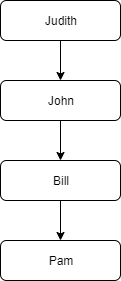
\includegraphics[scale=0.8]{family}
	\caption{Генеалогическое дерево}
\end{figure}

\subsubsection{Онтология}

Построим описание онтологии из примера на естественном языке. Программа определяет степень родства между людьми. Входными данными для программы являются:

\begin{itemize}
	\item Имя и пол человека.
	\item Родительские связи.
\end{itemize}

На основании этих данных программа определяет:

\begin{itemize}
	\item Если человек является родителем и мужчиной, то он -- отец.
	\item Если человек является родителем другого родителя и мужчиной, то он -- дедушка.
	\item Если человек связан цепочкой родительских связей с другим человеком, то они -- родственники.
\end{itemize}

\subsubsection{Концептуальная карта}

Построим концептуальную карту (семантическую сеть), описывающую данный пример.

\begin{figure}[H]
	\centering
	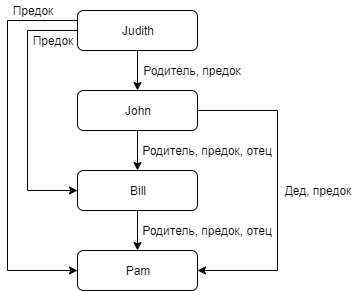
\includegraphics[scale=0.8]{map}
	\caption{Концептуальная карта}
\end{figure}

\subsection{Примеры из пособия}

\subsubsection{Географические субъекты}

В данном примере продемонстрированы особенности синтаксиса языка и формат описания правил. 

\prolog{project1}

Выведены все данные, полученные из предикатов \code{situ}. Например, выведен факт, что \code{warszawa - europe}, хотя этого факта нет в заданных предикатах.

\subsubsection{Составные объекты}

Данный проект иллюстрирует возможность использования составных объектов на языке Prolog.

\prolog{project2}

Видно, что был сконструирован составной объект книга, содержащий множество других полей, таких как название, автор и еще один составной объект -- публикация. Публикация в свою очередь включает издателя и год издания.

\subsubsection{Задача о семейных отношениях}

По исходным данным (Иван -- отец Игоря и Сидора; Сидор -- отец Лизы) необходимо выяснить,  есть ли брат у Игоря.

\prolog{project3}

Программа определила, что Сидор -- брат Игоря.

\subsubsection{Арифметические операции}

В данной программе реализуются собственные предикаты для определения суммы двух целых чисел, суммы двух вещественных чисел и максимума из трех вещественных чисел. 

\prolog{project4}

Видно, что суммы посчитаны, максимум определен.

\subsubsection{Использование анонимных переменных}

В данной программе используются анонимные переменные (\code{_}), значения которых безразличны для получения решения.

\prolog{project5}

Использование анонимных переменных не только упрощает процесс поиска решения, но и сокращает объем информации, получаемой пользователем.

\subsubsection{Явное указание цели}

В данной программе демонстрируется возможность использования пользовательских предикатов в качестве стандартных.

\prolog{project6}

Видно, что в качестве цели указан предикат \code{hello}.

\subsubsection{Предикат \code{fail}}

Предикат \code{fail} вызывает искусственное неуспешное завершение поиска, что позволяет получить все возможные решения задачи.

\prolog{project7}

Видно, что в результате были напечатаны названия всех городов.

\subsubsection{Предикат \code{cut} (1)}

Предикат \code{cut} позволяет получить доступ только к части данных, устраняя дальнейшие поисковые действия.

\prolog{project8}

Видно, что выведены только имена мальчиков, т.к. благодаря оператору \code{cut} (\code{!}) после имени Олег поиск прекращается.

\subsubsection{Предикат \code{cut} (2)}

Программа демонстрирует особенности работы оператора \code{cut}.

\prolog{project9}

Данная программа не находит ни одного решения, поскольку после дорогих зеленых <<жигулей>> (26000) поиск заканчивается, и более дешевые <<ауди>> (20000) не будут найдены, хотя удовлетворяют искомым параметрам.

\subsubsection{Рекурсия}

Данная программа демонстрирует использование механизма рекурсии в языке Prolog. 

\prolog{project10}

\noindent В разделе \code{clauses} программы даны два описания предиката \code{write_number}. Если в процессе решения первое описание неуспешно, то используется второе описание (рекурсивное).

\subsubsection{Сумма цифр числа}

Программа печатает сумму цифр числа, введенного в качестве аргумента в предикат \code{summa}, который рекурсивно ее вычисляет.

\prolog{project11}

Использование предиката \code{!} в описании нерекурсивного правила позволяет избежать здесь переполнения стека.

\subsubsection{Ханойская башня}

Требуется переместить диски с первого на третий стержень за некоторую последовательность ходов, каждый из которых заключается в перекладывания верхнего диска с одного из стержней на другой стержень. При этом больший диск никогда нельзя ставить на меньший диск.

\prolog{project12}

В результате выводится список действий, необходимых для решения данной задачи.

\subsubsection{Списки}

В программе демонстрируется использование списка в языке Prolog, с помощью которого обрабатываются породы собак.

\prolog{project13}

Операция разделения списка на голову и хвост обозначается с помощью вертикальной черты: \code{[Head} | \code{Tail]}. С помощью этой операции реализована рекурсивная обработка списка. В данном случае на консоль выводятся все элементы списка.

\subsubsection{Правило \code{find_it}}

Программа состоит из двух описаний правила \code{find_it}. Первое правило описывает ситуацию, когда искомый элемент Х совпадает с головой списка. Второе правило используется при неуспехе первого правила и описывает новый вызов первого правила, но уже с усеченным списком, в котором нет первого элемента и т.д. Если в списке нет элементов (пустой список), то второе правило оказывается неуспешным.

\prolog{project14}

Программа не напечатала <<Yes>>, поскольку <<Lapdog>> нет в списке собак.

\subsubsection{Сумма элементов списка}

Программа производит подсчет элементов списка и выводит результат в консоль. 

\prolog{project15}

Сумма элементов списка \code{[4, 4, 2, 5, 4, 3, 100]} равна \code{122}.

\subsubsection{Мужик, волк, коза и капуста}

Данная программа решает задачу о мужике, волке, козе и капусте. Для этого использованы списки и механизм рекурсии при их обработке.

\prolog{project16}

В консоль выводится решение -- последовательность действий, которые должен совершить мужик.

\subsubsection{Логическая задача (1)}

Программа решает простую логическую задачу распределения мест среди трех велосипедистов: <<В велосипедных гонках три первых места заняли Алеша, Петя и Коля. Какое место занял каждый из них, если Петя занял не второе и не третье место, а Коля – не третье?>>

\prolog{project17}

Видно, что задача решена верно, т.к. все условия задачи соблюдены.

\subsubsection{Логическая задача (2)}

Пятеро студентов едут на велосипедах. Их зовут Сергей, Борис, Леонид, Григорий и Виктор. Велосипеды сделаны в пяти городах: Риге, Пензе, Львове, Харькове и Москве. Каждый из студентов родился в одном из этих городов, но ни один из студентов не едет на велосипеде, сделанном на его родине.

\begin{itemize}
	\item Сергей едет на велосипеде, сделанном в Риге.
	\item Борис родом из Риги, у него велосипед из Пензы.
	\item У Виктора велосипед из Москвы.
	\item У Григория велосипед из Харькова.
	\item Виктор родом из Львова.
	\item Уроженец Пензы едет на велосипеде, сделанном на родине Леонида.
\end{itemize}

Кто из студентов родом из Москвы?

\prolog{project18}

Видно, что задача решена верно, т.к. все условия задачи соблюдены.

\subsubsection{Логическая задача (3)}

Пять студентов должны посещать лекции всю неделю, но по определенным ими установленным правилам, а именно:

\begin{enumerate}
	\item Если пришли Андрей и Дмитрий, то Бориса быть не должно, но если Дмитрий не пришел, то Борис должен быть, а Виктор быть не должен. 
	\item Если Виктор пришел, то Андрея быть не должно и наоборот. 
	\item Если Дмитрий пришел, то Григория быть не должно. 
	\item Если Бориса нет, то Дмитрий должен быть, но, если нет также и Виктора, а если Виктор есть, Дмитрия быть не должно, но должен быть Григорий. 
	\item Каждый день студенты должны приходить в разных сочетаниях. Какие это сочетания?
\end{enumerate}

\prolog{project19}

Видно, что задача решена верно, т.к. все условия задачи соблюдены.

\subsubsection{База данных}

В программе осуществляется поиск человека выше 180 см и выводится его фамилия, рост и вес. При этом факты, описанные в разделе \code{clauses}, рассмотрены как статическая база данных (БД). Эти факты являются частью кода программы и не могут быть оперативно изменены.

\prolog{project20}

Вывод программы соответствует поисковому запросу.

\subsubsection{Простая экспертная система}

Данная программа реализует простую экспертную систему, которая решает задачу определения вида экземпляра пойманной рыбы.

\prolog{project21}

Видно, что программа реализует заданное дерево поиска решения. Ответы на заданные вопросы позволяют продвигаться по ветвям этого дерева к одному из вариантов решения.

\section{Выводы}

В лабораторной работе рассмотрен язык логического программирования Prolog. Продемонстрированы его особенности: работа с предикатами, списками, создание пользовательских предикатов, использование механизма рекурсии. Разработано множество программ, решающих различные задачи. В процессе работы приобретены навыки работы в оболочке Visual Prolog.

\bibliographystyle{plain}
\addcontentsline{toc}{section}{Список литературы}
\bibliography{refs}

\end{document}
